We also evaluated the model as a predictor of reading times on the fillers.
We expected that the model should provide competitive model fit at least in some of the regions of the parameter space in which it also predicts reading times in center embeddings well.
Besides our Maze data, we also considered eyetracking and self-paced-reading data collected for these fillers by \cite{vasishth2010short}.

To account for spillover effects that are prominent in eyetracking and particularly self-paced reading, we include predictors from the preceding token in all reading measures.
We fitted log-transformed reading times for Maze and Self-Paced Reading, and raw reading times for Eye-Tracking\footnote{The rationale for this is that we use reading times from the preceding word as covariates to account for potential spillover effects. As reading times can be zero in eyetracking, log-transformation does not make sense there.}.

We constructed mixed-effects models with the following fixed effects:
\begin{enumerate}
	\item Model surprisal, averaged over all model runs at a given retention rate $\delta$\footnote{We found equivalent results when instead computing AIC for every model run individually, and then averaging for all runs at a given retention rate $\delta$.}
\item word length
\item Log word frequency in the British National Corpus \citep{Leech1992100MW}
\item Log word Frequency in the Corpus of Contemporary American English \citep[COCA][]{Davies2012TheCO}
\item The same predictors (1-4), and the corresponding reading time measure, for the preceding word
\end{enumerate}
We entered items (i.e., word tokens) and subjects as random effects.
Due to computational cost constraints, we created frequentist mixed-effects models using \texttt{lme4} \citep{Bates2014FittingLM} with random intercepts only.
We compared model fit using Akaike Information Criterion \citep[AIC][]{Akaike1973InformationTA}.

There are about 730 distinct tokens in 56 sentences.
For Maze, we have data from $>$700 subjects, each of which read 30 of 56 fillers. 
For the other modalities, we have considerably less data, both because \cite{vasishth2010short} recruited fewer participants, and because they used multiple lists of fillers, so that not every participant read each of the fillers used in our study.

We show model fit, measured using AIC, in Figure~\ref{figure:fillers-fit}.
We compare model fit to GPT-2, for which we clipped context length to 20 for fair comparison with the resource-rational model.
White cells indicate fit equivalent to vanilla GPT2.
Red cells indicate better model fit than vanilla GPT2; blue fit indicates poorer fit.
In all three modalities, model fit is at least competitive with vanilla GPT2 across a wide area in the parameter space:
In particular, model fit is at least as good as that of GPT2 whenver $\delta \geq 3$. 
There is also a clear overlap between the regions where model fit is best across the fillers with the regions where prediction is best for the final verb in center embeddings (compare Figure~\ref{fig:fit-critical}).
We also specifically compared model fit to Maze reading times between plain surprisal ($\delta=0$), and the configuration reported in Figure 3 of the main paper ($\delta=10$). 
The model strongly improved fit over plain surprisal ($\Delta$AIC = 24).



The success of our model in predicting reading times when retaining only half or less of context words explains recent findings that reading times are impacted by local statistics beyond surprisal~\citep{DBLP:journals/corr/abs-2103-04469} and that n-gram models provide relatively good fit to reading times compared to their limited statistical fit to language~\citep{DBLP:conf/cogsci/WilcoxGHQL20}.




While the model improves fit in all three modalities, the parameters leading to best fit in Eyetracking and Self-Paced Reading appear to have lower retention rates $\delta$ when compared to Maze.
This may suggest that participants tend to be less attentive in those paradigms than in Maze.

We considered whether the improvement over full surprisal can be localized to specific contexts or constructions, such as long dependencies. We found no evidence for such localized effects; instead, the improvement appears to be an across-the-board statistical improvement. Investigating this in more detail is an interesting question for future work.


\begin{figure}
	\centering

	Maze (251K observations) 

    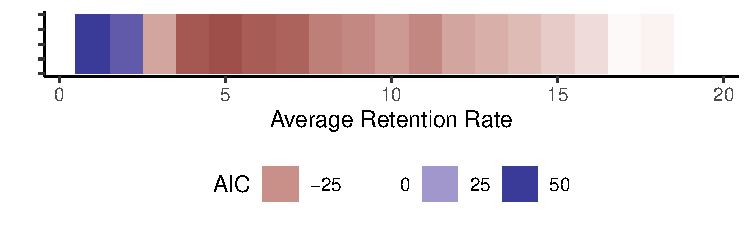
\includegraphics[width=0.5\textwidth]{../resource-rational-surprisal/model/compute_surprisal/analyze_output/fillers/figures/analyzeFillers_freq_BNC_Spillover_Averaged_New_R_Lambda1_Integer.pdf}

	Eye-Tracking (First Pass Reading Times, 7K observations) 

    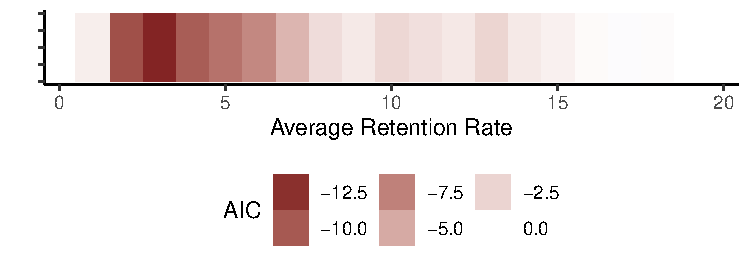
\includegraphics[width=0.5\textwidth]{../resource-rational-surprisal/model/compute_surprisal/analyze_output/fillers/figures/analyzeFillers_freq_BNC_FPRT_Spillover_Averaged_New_R_Lambda1_Integer.pdf}

	Self-Paced Reading (26K observations) 

    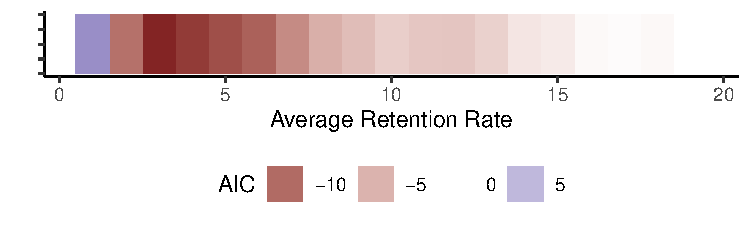
\includegraphics[width=0.5\textwidth]{../resource-rational-surprisal/model/compute_surprisal/analyze_output/fillers/figures/analyzeFillers_freq_BNC_SPR_Spillover_Averaged_New_R_Lambda1_Integer.pdf}


	\caption{Model fit on reading times on the fillers. Eye-tracking and self-paced reading data was collected by \cite{vasishth2010short}. We show the AIC difference compared to pure GPT2; negative values indicate better model fit. The model improves over GPT2 over a wide range of retention rates. Low retention rates seem to lead to better model fit in eye-tracking and self-paced reading than in Maze, potentially suggesting lower attention in those paradigms. 
	}\label{figure:fillers-fit}
\end{figure}


\paragraph{Including DLT}
We further added DLT integration cost as a predictor into the analyses.
We operationalized this as follows based on \citet{Demberg2008DataFE}.
We parsed the fillers using Stanza \citep{Qi2020StanzaAP} into the Universal Dependencies 2 format, a standard representation format for syntactic dependencies.
We treated nouns (NOUN and PROPN) and verbs (VERB) as introducing discourse referents.\footnote{We did not treat AUX as introducing a discourse referent because \citet{Demberg2008DataFE} found a \emph{facilitating} effect of intervening auxiliaries, opposite to the DLT prediction if they are treated as discourse references.}
As \citet{Demberg2008DataFE} analyzed effects on nouns and verbs separately, we created separate predictors for nouns and verbs. These were centered within the relevant POS category (nouns or verbs), and then set to zero for other words.\footnote{We found equivalent results when zeroing them for other words \emph{before} centering.}
With the DLT predictors, the model continued to improve over plain surprisal ($\Delta AIC = -23$ for $\delta=10$ vs full surprisal) in fitting the Maze data.

